\chapter{Virtualization and Containerization} \label{ch:vac}

Virtualization and containerization are widely appreciated technologies for distributing multiple instances of applications on single or multiple physical servers. 

The primary objective of these technologies is to enhance resource utilization efficiency while ensuring isolation between applications. Containerization is also found useful in fast migration and deployment of applications on new platforms.

\section{Introduction}

One of the major differences between a server and a PC is that the former is usually shared among multiple users or applications at the same time. Though working on the same machine, a user would usually want a private working environment not interrupted by other users. In other words, a user would want to ``virtually'' work on an independent machine with his own CPU, RAM, I/O, OS, drivers and storage, despite that the actual hardware is shared with others. 

This can be achieved through \mync{virtualization}, which enables running multiple operating systems on a single physical server in an uninterrupted and logically separated manner. The virtually independent computer of such kind is often called a \mync{virtual machine}[VM].

Deploying a new VM generally consumes a considerably large amount of time and resources. This is because different VMs on the same server are separated at the OS level, with each VM requiring its own OS installation. Consider a scenario where there are hundreds of small applications (microservices), each requiring a similar but separate environment. Launching VMs for each and every of them is resource-intensive and can become an unnecessary waste of resource when these applications could have shared the same OS kernel and operated within their own isolated workspace.

In the above scenario, a more efficient approach is to deploy a single VM and place each application in a ``container'' with its own customized drivers and configurations. A container is similar to a VM in the sense that it provides a degree of isolation from others, but it is typically ``lighter'' than a VM because it doesn't need to virtualize or duplicate the whole OS as VMs do. This makes containers cheaper to launch and manage.

The technology used to deploy and manage containers is known as \mync{containerization}. A container contains all the configuration and requirement information of an application. Running a container on different platforms would consistently generate the same expected result. This has made the sharing and rapid deployment of containers remarkably easy and convenient. The similarities and differences of personal PCs, VMs, and container applications are summarized in Fig. \ref{ch:vac:fig:pcvmcontainersructure}.

\begin{figure}[!htb]
	\centering
	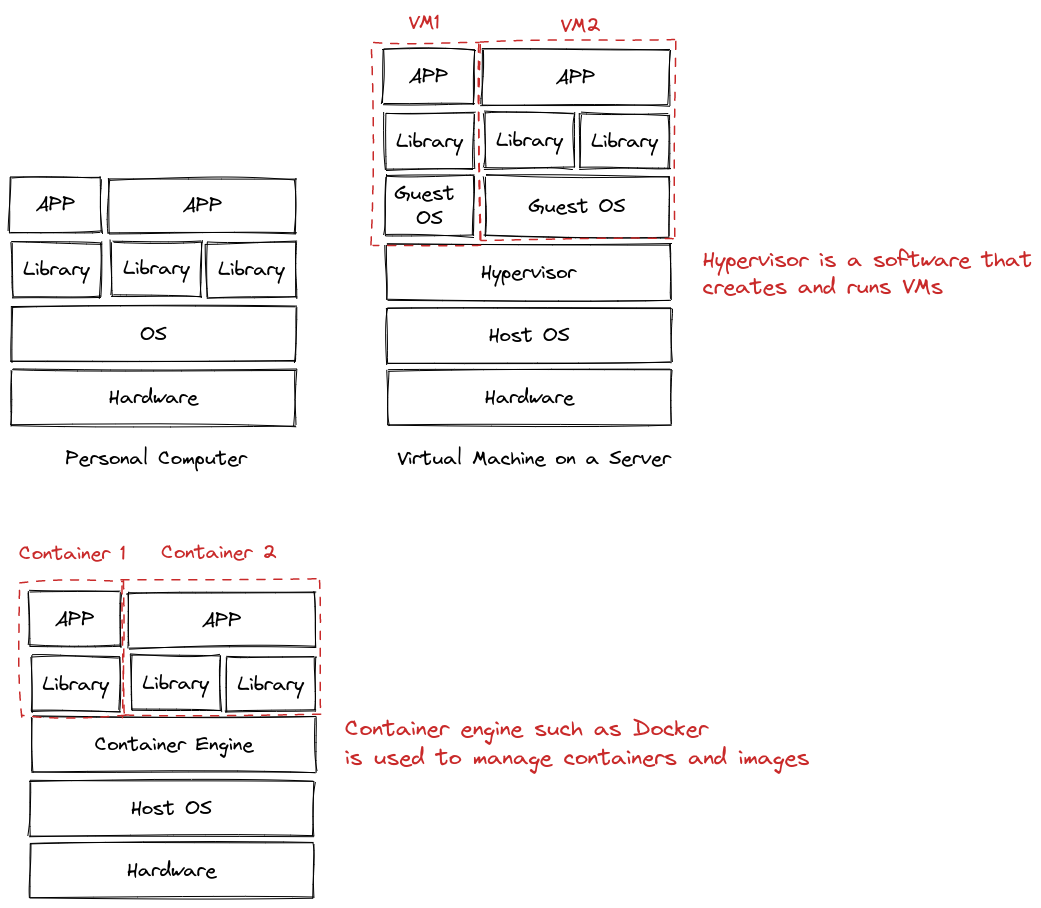
\includegraphics[width=350pt]{chapters/part-3/figures/pcvmcontainerstructure.png}
	\caption{System architectures of PC, VM and container.} \label{ch:vac:fig:pcvmcontainersructure}
\end{figure}

As an analogy, think of running an APP as cooking a dish. The hardware corresponds with the physical resources in the kitchen such as the cooktop and gas. The OS corresponds with the cook. The OS requires drivers and libraries to run the APP correctly. The drivers and libraries correspond with the specific skills or cookers for the dish. Finally, the APP is corresponding with the expected dish.

In the most simple configuration, a dedicated machine is used to run an APP. This is like constructing a dedicated kitchen and hiring a dedicated cook for each dish. The cook is trained to master all necessary skills required for that specific dish. This is shown in Fig. \ref{ch:vac:fig:acookinakitchen}.
\begin{figure}[htbp]
	\centering
	
\includegraphics[width=300pt]{chapters/part-3/figures/acookinakitchen.png}
	\caption{PC implementation: a cook in a kitchen.} \label{ch:vac:fig:acookinakitchen}
\end{figure}

In a VM implementation, a large and capable kitchen is setup in advance as shown in Fig. \ref{ch:vac:fig:manycooksinakitchen}. For each dish, a cook is hired. Each cook is trained with the skills necessary for his assigned dish. All cooks share the same kitchen. This implementation is more efficient than Fig. \ref{ch:vac:fig:acookinakitchen}, as there is no need to scale up the kitchen for a new dish. By sharing the resources among the cooks, the kitchen can be utilized more efficiently.
\begin{figure}[htbp]
	\centering 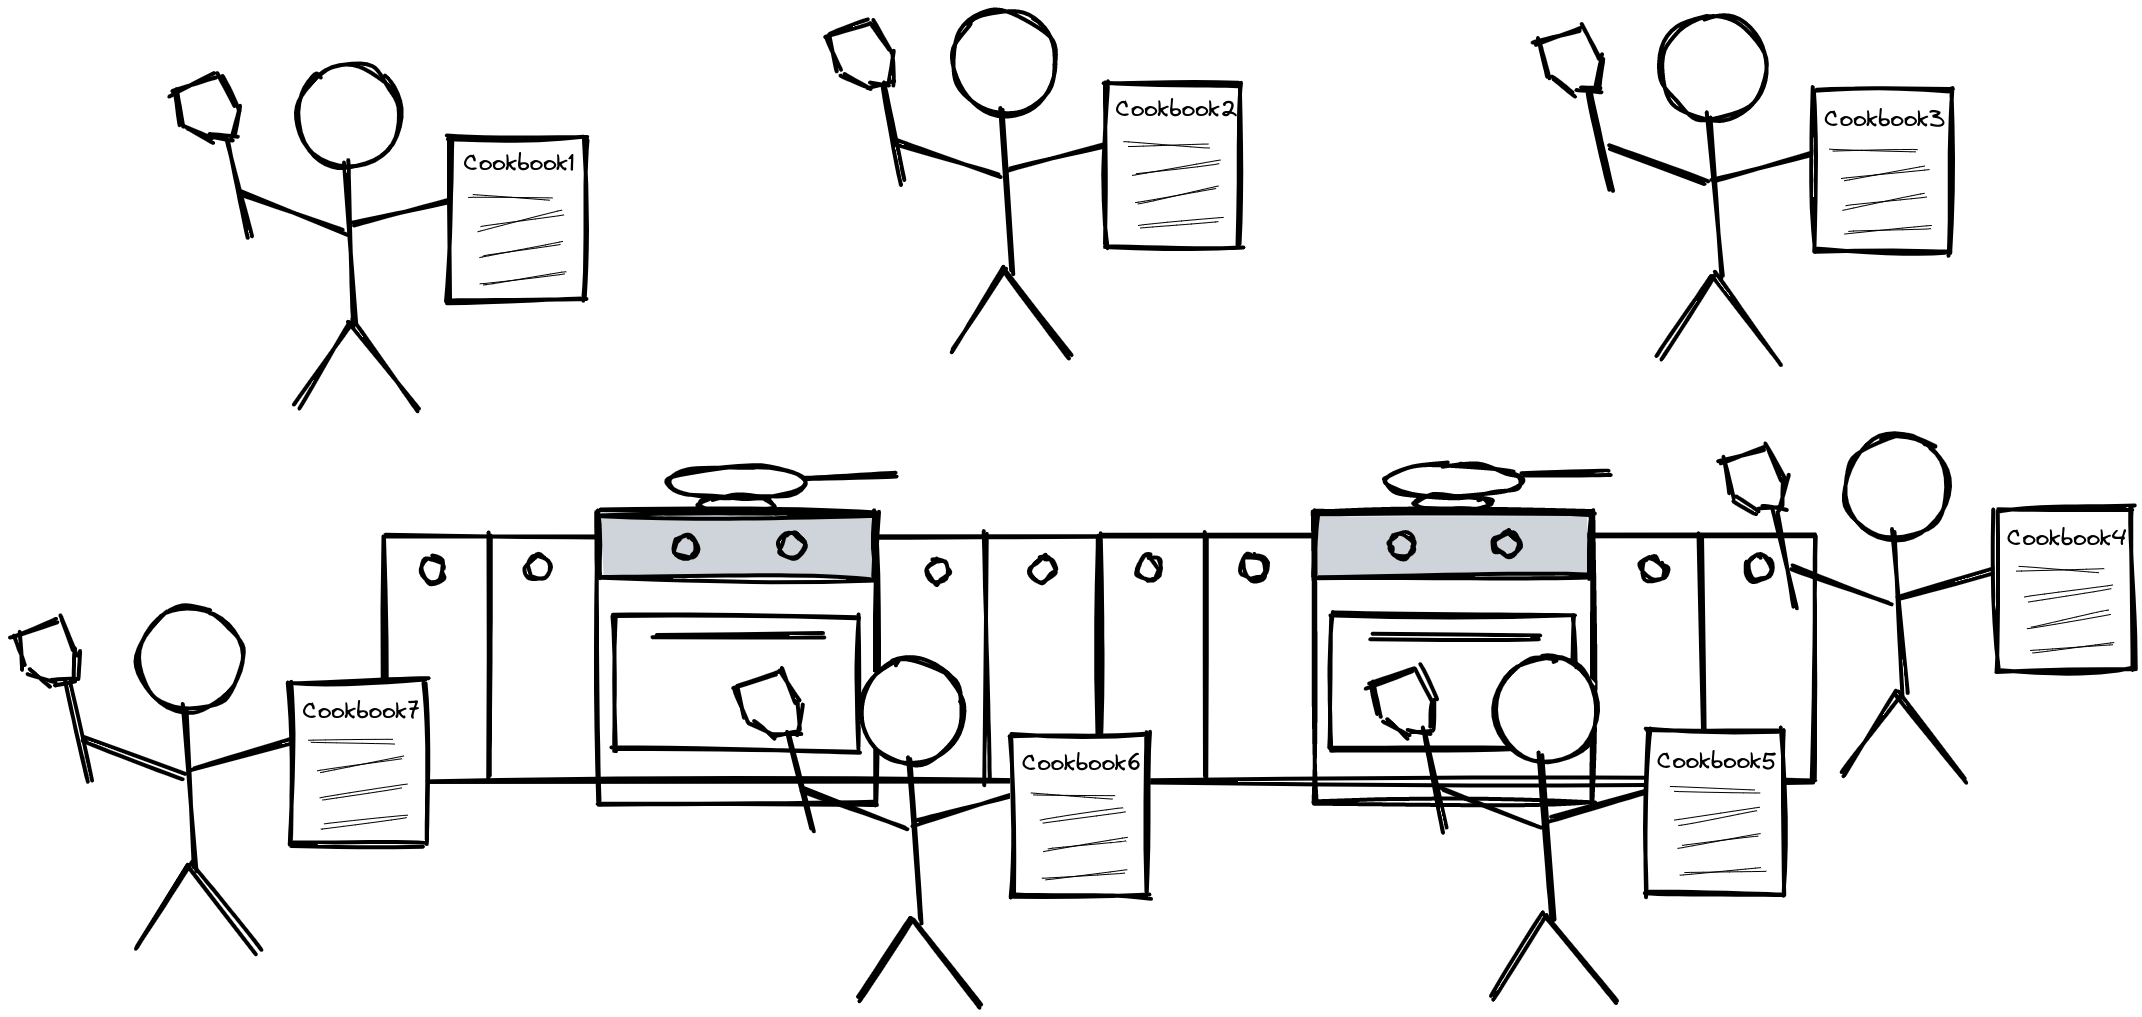
\includegraphics[width=350pt]{chapters/part-3/figures/manycooksinakitchen.png}
	\caption{VM implementation: many cooks in a kitchen, each with a different cookbook.} \label{ch:vac:fig:manycooksinakitchen}
\end{figure}

While Fig. \ref{ch:vac:fig:manycooksinakitchen} might be a popular practice in many restaurants, it is still too costly to hire a new cook for each dish. In a containerization implementation, a cook usually handles a category of dishes, as shown in Fig. \ref{ch:vac:fig:multitaskcook}. Of course, each dish will stay in its own fry-pan in an isolated way. For each dish, its recipe is provided that gives all information required to prepare the dish consistently. As long as the cook is good at multi-tasking and has the basic skill sets for general dishes, Fig. \ref{ch:vac:fig:multitaskcook} is usually a more efficient implementation than Figs. \ref{ch:vac:fig:acookinakitchen} and \ref{ch:vac:fig:manycooksinakitchen}.

\begin{figure}[htbp]
	\centering
	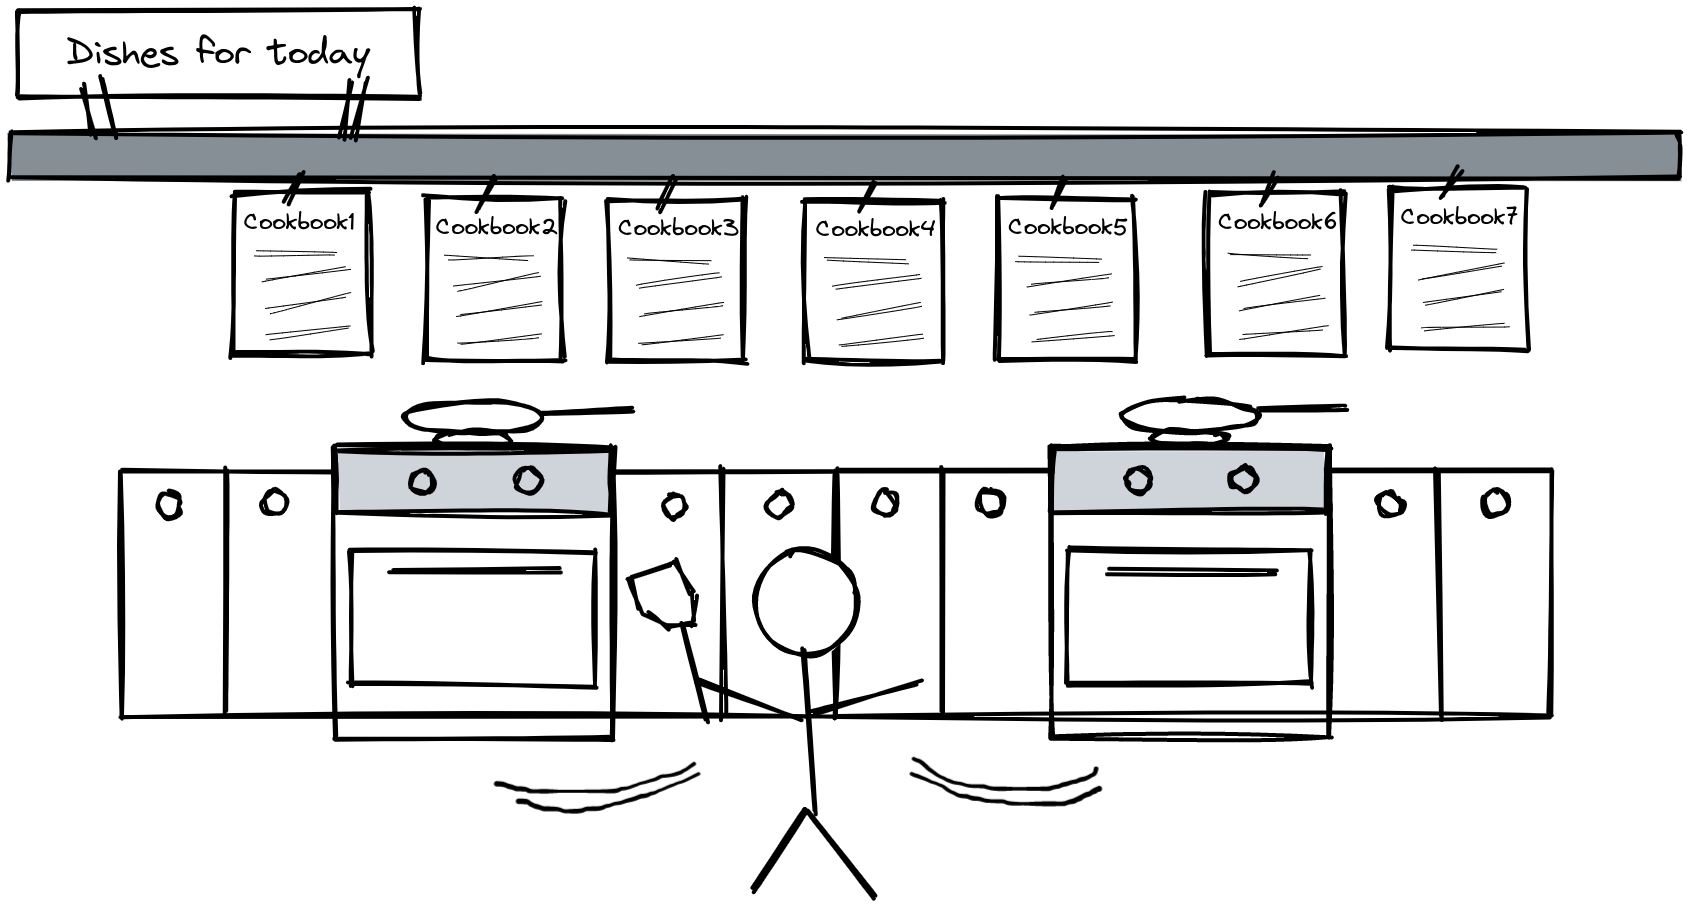
\includegraphics[width=350pt]{chapters/part-3/figures/multitaskcook.png}
	\caption{Container implementation: one cook in a kitchen, handling multiple dishes, each has a cookbook and stays in its own pan.} \label{ch:vac:fig:multitaskcook}
\end{figure}

Just like a recipe guaranteeing the consistency of dishes, in containerization, an ``image'' guarantees the consistent behavior of container instances. An image is basically a collection of prerequisites and configurations to start a container efficiently and consistently. Images can be shared among machines to replicate the containers even if the machines adopt different underlying infrastructures such as hardware and OS.

\section{Virtualization and Containerization}

Virtualization and containerization have been studied for decades. This section gives a brief introduction to both technologies.

\subsection{Virtualization}

In a conventional data center, multiple physical servers are deployed, and each server has a single associated application. Servers may share the same \myabb{local area network}{LAN} and \myabb{network-attached storage}{NAS} for data exchanging. A big issue of this implementation is the utilization efficiency of the servers and the unevenly distributed loads: some of the servers may not be utilized efficiently, while others may be overwhelmed. To deploy a new application, a new server must be purchased, which can take months of time. With more and more servers, the management and IT cost may grow exponentially.

To solve this problem, we need a systematical and automated way of integrating the resources in a data center and re-distributed them to the applications in an efficient manner. Virtualization is one of the most important technology used in this framework. Virtualization is essentially about running a system on a ``virtualized machine'', where by saying ``virtualized'' we mean that the machine is not a physical machine, but a virtual execution environment that is emulated and managed by a special software running on the actual machine known as the ``\mync{Virtual Machine Monitor}[VMM]'' or ``\mync{hypervisor}''. The setup should be transparent to the applications in the sense that the applications perform the same way as if it were running on a dedicated physical machine.

Depending on the items to be virtualized, virtualization can be divided into the following categories.
\begin{itemize}
  \item Virtualization of equipment, mainly network resources and storages. This results in \myabb{virtual LAN}{VLAN}, \myabb{virtual private network}{VPN}, NAS and \myabb{storage area network}{SAN}.
  \item Virtualization of operating systems. This results in the well-known VM and virtual desktop.
  \item Virtualization of application running environments. An example is \myabb{Java virtual machine}{JVM} that allows Java to generate consistent result while running on different machines.
\end{itemize}

There are different virtualization architectures. Commonly seen components shared by different architectures often include
\begin{itemize}
	\item Host OS. The OS that resides on the physical machine, on which virtualization tools run.
	\item VMM. This is a software that runs on the host OS, managing all the guest OSs, providing them interface to the host OS and the hardware.
	\item VM, the system that runs in an virtualized isolated environment.
\end{itemize}
Host OS, VMM and VM relationship is shown in Fig. \ref{ch:vac:fig:acookinakitchen}.

Different virtualization techniques are used in different types of VMMs. They can be widely divided into the following categories.
\begin{itemize}
	\item Full virtualization. The VMM virtualizes everything including the hardware. The guest OS can run on the VM without modification or adaptation, just like running on any other machine.
	\item Para-virtualization. The VMM does not virtualize hardware. The guest OS is modified to certain extent to suit the VMM of this type.
	\item Hardware-assisted virtualization. The processor of the system is specifically designed to provide certain VM functions. These functions, after passing through VMM, are directed and executed on the hadrware, thus enhancing system performance.
\end{itemize}

VMM is able to virtualize hardware resources such as CPU, memory and I/O. For the virtualization of CPU, the key is to virtualize privileged instructions (a set of instructions that can only be executed by software running in privileged mode, usually the OS) for the guest OS, so that the guest OS would think it is directly talking to a CPU. This is challenging because guest OS usually does not possess the privilege due to the VM architecture. If the requests of the guest OS contain privileged instructions, the CPU will deny the request. When that happens, an exception will be raised to the VMM which will take care of the privileged instructions sequentially. Since hypervisor runs in privileged mode, it can execute those instructions.

For the virtualization of memory, VMM uses shadow page table to assign memory pages to different VMs. The maximum memory allocated to a VM can change dynamically.

For the virtualization of I/O, the development trend is that I/O operations will be less and less rely on software and OS, and more and more on hardware. The VMM directly maps the I/O hardware interface to the VMs.

\begin{shortbox}
	\Boxhead{Hypervisor VS Host OS, Who is the Boss?}
	Both the hypervisor and the host OS can run in privilege mode (also known as ``Ring 0'' in x86 architecture). However, notice that at one time there can be only one boss, i.e., there can be only one entity that runs in Ring 0 at the same time.
	
	Depending on the type of the hypervisor configuration, this entity can be either the hypervisor or the host OS. In a type 1 hypervisor configuration, the hypervisor itself runs in Ring 0 and manages all hardware resources directly. In a type 2 hypervisor configuration, the host OS runs in Ring 0, and the hypervisor runs in a lower privileged ring.
\end{shortbox}

\subsection{Containerization}

Containerization is an alternative virtualization approach to VM that can also virtualize independent workspaces for applications. Comparing with VM, containers are often lighter, hence more efficient for massive microservices deployment. Depending on the context, the term ``container'' may refer to one or more of the following 3 concepts: container runtime, container engine, and container orchestration.

Container runtime refers to the backend software that actually executes the containers. Examples of widely used container runtimes are ``containerd'', ``runc'' and ``cri-o''. 

It is often inconvenient for users to talk to container runtimes directly. Container engine is the interface for a user or software to manage images and containers. Examples of container engines include ``docker'' and ``podman''. 

Finally, container orchestration is the software that strategically deploy, monitor, restart, and terminate the containers on servers. It can scale up and down the number of containers based on the demanding, and balance the API calls each container receives. Container orchestration is very useful in production environment of large-scale services. One of the most widely used container orchestrations is ``kubernetes''.

Notice that though container runtime is always a must-have, container engine and container orchestration are not.

\section{Docker Container Basics} \label{ch:vac:sec:dc}

This section introduces docker. Notice that though being famous for docker container engine, docker as a company or community provides many revolutionary container related tools and services that go far beyond a container engine brand. Many tools and technologies of docker are used in container runtimes and container engines of other brands.

This section focuses mostly on the introduction of docker container engine.

\subsection{Docker Engine VS Alternatives}

Docker engine is the most popular container engine available on the market as of 2023, and it is free of charge for open-source, personal and small business usage. More details of docker can be found at \textit{https://docs.docker.com/}.

But does that mean docker engine is the absolutely best and perfect container engine solution?

Docker has surely revolutionized how we use containerization technology in software development and deployment, and it has been one of the most popular and beloved container engine solutions. However, it is worth mentioning that docker engine is not the only available container engine. For example, as explained earlier podman is an alternative to docker. It supports the same interface as docker in its CLI (as if podman were an alias), and claims to have better performance and security. As a matter of fact, RHEL already started the transition from docker to podman from RHEL 8. Nowadays, installing docker on the latest versions of RHEL is possible but tedious. On the other hand, installation of podman on RHEL, if it had not been pre-installed, can be done simply by
\begin{lstlisting}
$ sudo dnf install podman
\end{lstlisting}
Kubernetes, a famous container orchestration, is also dropping docker support according to their statement ``docker support in the kubernetes is now deprecated and will be removed in a future release''. Some may even argue that ``containers are alive, but the role that docker plays is shrinking''. Many open-source initiatives such as podman are gaining popularity.

Docker has some disadvantages indeed. For one thing, docker uses docker server (docker daemon), a single piece of software running in the backend of the system, to support all the services. This creates a single-point-of-failure in the system. Docker requires root privileges, and it starts a container on behalf of the root user. This means that the program running inside the container and the users in the docker group can potentially bypass the OS access control and gain root access, which introduces security risk. These shortages are to some extent addressed by other container engines such as podman which is daemon-less and does not necessarily need to run on root user's behalf.

This is not to say that Docker is falling behind as a whole. Some key techniques that docker introduced are widely used in all different types and brands of container runtimes and engines. It is just that people do not like some of the features of docker engine, and alternative tools are being developed to fix these problems, the latter of which starting drawing more and more attention. Docker still enjoys widespread usage and support due to its massive community, wealth of online resources, and extensive compatibility with numerous tools and platforms. Nevertheless, for demonstration purpose, for the remaining sections docker is used throughout this notebook. Since podman provides the same interface, it is probable that podman can be used likewise to replicate all the results.

As of 2023, docker is still the dominating container market engine, with a market share of over $80\%$.

\subsection{Docker Installation}

To install docker on a Linux machine, go to \textit{https://www.docker.com/} to look for the instruction. The installation steps differ depending on the host machine. As explained earlier, RHEL uses podman as its recommended container engine, and podman comes with RHEL installation. 

In this section, consider installing docker engine on Ubuntu. Some of the key steps are summarized as follows. Remove existing docker engine, if any.
\begin{lstlisting}
$ sudo apt-get remove docker docker-engine docker.io
$ sudo apt-get remove containerd runc
\end{lstlisting}
Add docker's official GPG key and set up the repository.
\begin{lstlisting}
$ sudo apt-get update
$ sudo apt-get install ca-certificates curl gnupg lsb-release
$ sudo mkdir -p /etc/apt/keyrings
$ curl -fsSL https://download.docker.com/linux/ubuntu/gpg | sudo gpg --dearmor -o /etc/apt/keyrings/docker.gpg
$ echo \
  "deb [arch=$(dpkg --print-architecture) signed-by=/etc/apt/keyrings/docker.gpg] https://download.docker.com/linux/ubuntu \
  $(lsb_release -cs) stable" | sudo tee /etc/apt/sources.list.d/docker.list > /dev/null
\end{lstlisting}
Install docker.
\begin{lstlisting}
$ sudo apt-get update
$ sudo apt-get install docker-ce docker-ce-cli containerd.io docker-compose-plugin
\end{lstlisting}
where notice that \verb|docker-compose| is a toolkit to manage containers using CLI. It is a handy tool in the testing environment.

To test whether docker is installed correctly, run
\begin{lstlisting}
$ sudo docker run hello-world
\end{lstlisting}
and if everything is done correctly, a message started with ``Hello from Docker!'' will be displayed in the console, together with a brief introduction to how docker works.

Notice that to use docker commands, sudo privilege is required. To avoid typing \verb|sudo| each time running a docker command, add the user to the docker group as follows. In the rest of the section, \verb|sudo| is neglected for docker commands.
\begin{lstlisting}
$ sudo usermod <user name> -aG docker
\end{lstlisting}

Docker installs at least two piece of software on the machine, namely docker CLI and docker server. The CLI is the interface to the user, and the server the daemon. Docker runs natively on Linux OS. If docker is installed on non-Linux system such as Windows or macOS, ``docker desktop'' is used which includes a Linux VM to host the docker daemon and run Linux-based containers.

\subsection{Docker Container Management}

This section discusses basic container manipulation such as launching and stopping a container.

\vspace{0.1in}
\noindent \textbf{Launch}
\vspace{0.1in}

To create and run a container from an image, simply use
\begin{lstlisting}
$ docker run <configuration> <image>
\end{lstlisting}
Docker will search the local and remote repositories for the image, download the image if necessary, and start a container from that image. By default, \verb|docker run| starts a container in attached mode (frontend mode) unless flag \verb|-d| is used. After successful execution and completion of all the tasks, the container will enter ``Exited'' status. 

For example, consider running a container of \textit{alpine} using the command below. A screen shot is given in Fig. \ref{ch:vac:fig:dockerrunexp}.
\begin{lstlisting}
$ docker run -it --name test-alpine alpine
\end{lstlisting}
where \verb|-i| stands for ``interactive'', which keeps the container's standard input (i.e., the console in this example) open so that the user can actively interact with the container. Option \verb|-t| allocates a pseudo-TTY to the container. TTY stands for ``TeleTYpewriter'', which enforces the I/O of the container to follow the typical terminal format and allows the user to interact with the container like a traditional terminal, hence making the interactive interface a bit more user-friendly. Flags \verb|-it| are often used when running a container in attached mode. Finally, \verb|--name| assigns a name to the container. Without an assigned name, docker will assign a random name to the container.
\begin{figure}[!htb]
	\centering
	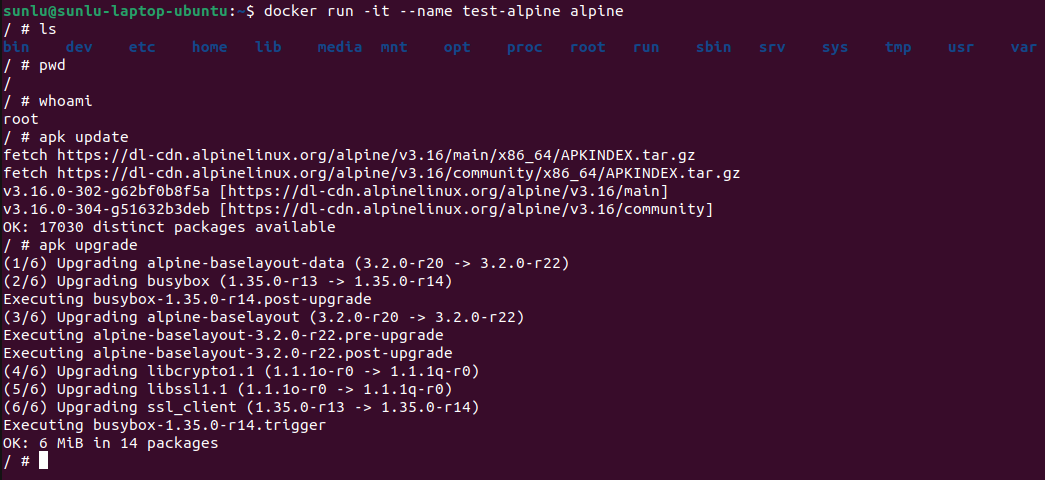
\includegraphics[width=350pt]{chapters/part-3/figures/dockerrunexp.png}
	\caption{An example of running \textit{apline} container, with interactive TTY and name \textit{test-apline}.} \label{ch:vac:fig:dockerrunexp}
\end{figure}

It can be seen from Fig. \ref{ch:vac:fig:dockerrunexp} that once the container is started, the user can interact with the container via shell and perform actions such as listing items in the current directory in the container. This is because the container is running in attached mode, and flags \verb|-it| map the the containers input and output with the console.

While keeping the container running, open another terminal and use \verb|docker container ls| to check the status of the container. More about \verb|docker container ls| are introduced later. The container \verb|test-alpine| shall appear in the list, as shown in Fig. \ref{ch:vac:fig:dockerrunexppart2}.
\begin{figure}[!htb]
	\centering
	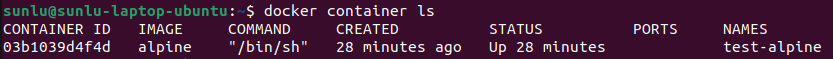
\includegraphics[width=250pt]{chapters/part-3/figures/dockerrunexppart2.png}
	\caption{List the running container \textit{test-apline}.} \label{ch:vac:fig:dockerrunexppart2}
\end{figure}
After exiting from Fig. \ref{ch:vac:fig:dockerrunexp} (by using \verb|exit| in \textit{alpine}), the container will transfer its status from ``running'' to ``exited'', as shown in Fig. \ref{ch:vac:fig:dockerrunexppart3}.
\begin{figure}[!htb]
	\centering
	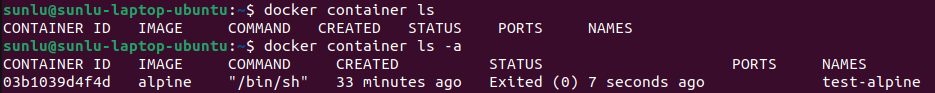
\includegraphics[width=250pt]{chapters/part-3/figures/dockerrunexppart3.png}
	\caption{List the exited container \textit{test-apline}.} \label{ch:vac:fig:dockerrunexppart3}
\end{figure}

Functional wise, \verb|docker run| executes two commands behind the screen, namely \verb|docker create| and \verb|docker start|, where \verb|docker create| creates a container and \verb|docker start| starts the container by executing the startup script defined in the image. These two commands can be used separately. For example, to start an exited container, use
\begin{lstlisting}
$ docker start <container>
\end{lstlisting}

\begin{shortbox}
\Boxhead{Differences between \texttt{docker run} and \texttt{docker start}}

Do note the fundamental differences between \verb|docker run| and \verb|docker start|. First of all, \verb|docker run| starts a container from an image and it always creates a new container, whereas \verb|docker start| starts an existing but exit container. Secondly, \verb|docker run| runs a container in attached mode by default unless \verb|-d| flag is used, while in contrast \verb|docker start| runs a container in detached (backend) mode by default unless \verb|-a| is used. 
\end{shortbox}

An example of using \verb|docker run| with \verb|-d| flag to start a container in detached mode is given below.
\begin{lstlisting}
$ docker run -d --name test-background-alpine alpine
\end{lstlisting}
By changing \verb|-it| to \verb|-d|, the container runs in the backend silently. The status of the container, after executing the above command, will stay running and can be displayed by \verb|docker container ls|.

Commonly used commands regarding launching a container are given in Table \ref{ch:vac:tab:launchcontainer}.

\begin{table}[!htb]
	\centering \caption{Commonly used docker commands to launch a container.}\label{ch:vac:tab:launchcontainer}
	\begin{tabularx}{\textwidth}{llX}
		\hline
		Command & Flag & Description \\ \hline
		\verb|docker run| & --- & Launch a container from an image in attached mode by default. If the image cannot be found locally, it downloads the image from the remote repository automatically. \\
        \verb|docker start| & --- & Start an existing but exit container in detached mode by default. \\
        \verb|docker run| & \verb|-i| & Keep the standard input of the container open when launching the container. \\ 
        \verb|docker run| & \verb|-d| & Launch the container in the backend and keep it running. \\ 
        \verb|docker run| & \verb|--rm| & Automatically remove the container when exiting. The removed container will not be listed in \verb|docker container ls -a|. This is usually used with temporary containers during debugging. \\ 
        \verb|docker run| & \verb|-t| & Allocate a pseudo-TTY. The flag usually comes with the flags \verb|-i| or \verb|-d|, to form \verb|-it| or \verb|-dt|. \\ 
        \verb|docker run| & \verb|--restart| & Enforce restart of the container upon exiting. This is usually used on containers running in the backend. Commonly used restart configurations include \verb|--restart no| (do not restart), \verb|--restart on-failure[:<max retries>]| (restart if exits with an error flag), \verb|--restart always| (always restart when exists). \\ 
        \verb|docker run| & \verb|--name| & Assign a name to the container. \\
		\hline
	\end{tabularx}
\end{table}

It is worth mentioning that file system snapshot and startup commands are defined inside an image. See Section \ref{ch:vac:sec:di} for more details. When a container starts, the file system snapshot is pasted to the container file system, and the startup commands executed. It is possible to overwrite the startup commands when starting a container, simply by amending the revised startup commands to the image name as follows.
\begin{lstlisting}
$ docker run <image> <revised command>
\end{lstlisting}
where \verb|<revised command>| must be defined in the image, or otherwise an error will be raised.

\vspace{0.1in}
\noindent \textbf{Interaction}
\vspace{0.1in}

For a container running in the backend, use \verb|docker exec| to execute a shell command in that container as follows.
\begin{lstlisting}
$ docker exec <container> <command>
\end{lstlisting}
To enable the TTY shell of a container running in the backend, use
\begin{lstlisting}
$ docker exec -it <container> <command>
\end{lstlisting}
If \verb|<command>| is replaced by the shell name used in the container, this would open the terminal of the container. Notice that the shell used by the application running inside the container may differ from the one used in the host machine. In the case of an \textit{alpine} image based container, \verb|ash| is the default shell. For a \textit{ubuntu} image based container, \verb|bash| is often used. To exit from the TTY shell while keep the container running in the backend, use shortcut key \verb|Ctrl+p+q|. An alternative way to interact with containers running in the backend is to use
\begin{lstlisting}
$ docker attach <container>
\end{lstlisting}
to attach local standard input, output, and error streams to a running container. Similar with the previously introduced \texttt{docker exec -it} command, \texttt{docker attach} also starts the shell of the application running in the container. Use \verb|Ctrl-C| to quite the shell.

\vspace{0.1in}
\noindent \textbf{Stop and Removal}
\vspace{0.1in}

To stop, kill or restart a container running in the backend, use
\begin{lstlisting}
$ docker stop <container>
$ docker kill <container>
$ docker restart <container>
\end{lstlisting}
respectively. The difference between \verb|docker stop| and \verb|docker kill| concerns with how the OS manages process. When \verb|docker stop| is used, a  \verb|SIGTERM| signal is sent to the main process that the container runs. The container still has a little bit of time (maximum $10$ seconds) to terminate the job and clean up. When \verb|docker kill| is used, \verb|SIGKILL| signal is sent to the process, and the process is terminated immediately. When a container is stopped, it enters exited status.

To remove an exited container, use
\begin{lstlisting}
$ docker (container) rm <container>
\end{lstlisting}
where \verb|container| can be neglected. Alternatively, use
\begin{lstlisting}
$ docker container prune
\end{lstlisting}
to remove all exited containers. Notice that there is a more powerful command
\begin{lstlisting}
$ docker system prune
\end{lstlisting}
which removes not only exited containers but also unused network configurations, dangling images and cache.

\vspace{0.1in}
\noindent \textbf{Rename}
\vspace{0.1in}

To rename a container (without changing its container ID or anything else), use
\begin{lstlisting}
$ docker rename <container-old-name> <container-new-name>
\end{lstlisting}

\vspace{0.1in}
\noindent \textbf{Monitoring}
\vspace{0.1in}

Use
\begin{lstlisting}
$ docker container ls
\end{lstlisting}
to check the list of running containers, and
\begin{lstlisting}
$ docker container ls -a
\end{lstlisting}
the list of all containers, running or exited. Alternatively, \verb|docker ps|, \verb|docker ps -a| can also be used to list down containers just like \verb|docker container ls|, \verb|docker container ls -a|.

To check the processes that is running in the container, use
\begin{lstlisting}
$ docker top <container>
\end{lstlisting}

To quickly check container status including resource consumption (CPU, memory usage, etc.), use
\begin{lstlisting}
$ docker stats [<container>]
\end{lstlisting}
where the user can choose to list down all containers or a specified container. To show more detailed information of a container, including its status, gateway, IP address, etc., use
\begin{lstlisting}
$ docker inspect <container>
\end{lstlisting}
Finally, to check the logs of a container such as its standard output or error message, use
\begin{lstlisting}
$ docker logs <container>
\end{lstlisting}

\vspace{0.1in}
\noindent \textbf{File Exchange with Host Machine}
\vspace{0.1in}

There are multiple ways and protocols to access the files in a container, depending on the I/O setup of the container. For a container running locally, \verb|docker cp| can be used for file transfer between the container and the host machine as follows. From container to host machine:
\begin{lstlisting}
$ docker cp <container>:<source> <destination>
\end{lstlisting}
and from host machine to container:
\begin{lstlisting}
$ docker cp <source> <container>:<destination>
\end{lstlisting}
where \verb|<source>| and \verb|<destination>| refer to the path to the source and destination, respectively, located in the host machine or the container.

\vspace{0.1in}
\noindent \textbf{Commit}
\vspace{0.1in}

A container is usually generated from an image. It is also possible to do vise versa, i.e., packaging a container into an image. Notice that this is generally not recommended. Images shall be created mostly from Dockerfile, as will be introduced in Section \ref{ch:vac:sec:di}.

To create an image from a container, use
\begin{lstlisting}
$ docker commit <container> <image>
\end{lstlisting}
or
\begin{lstlisting}
$ docker commit -c 'CMD ["<startup command>"]' <container> <image>
\end{lstlisting}
where \verb|docker commit| command saves the container's file changes or settings into a new image, which allows easier populating containers or debugging in a later stage. Notice that \verb|docker commit| does not save everything of the container into the image, and it is not the only way an image is created.

\vspace{0.1in}
\noindent \textbf{Ports Publishing}
\vspace{0.1in}

By default, containers do not expose any ports to the outside world. A container can be accessed only from its host machine using APIs provided by docker, such as \verb|docker cp| to transfer files and \verb|docker exec| to execute commands, but not network protocols. The user can allow public access from the internet by publishing the ports of the container using
\begin{lstlisting}
$ docker run -p <host machine port>:<container port> <image>
\end{lstlisting}
when starting a container. To publish multiple ports, use multiple \verb|-p| flags in a command.

More about containerized application connectivity to the internet, to the host machine and to other containerized applications are introduced in later sections.

\subsection{An Example: Deploy a Containerized Application}

An example of setting up a web server in containers from scratch is given in this section. For simplicity, everything happens on a single physical server. Only one container is used and the load balancer and the shared services are not included in the example.

As a first step, create a container from the official \textit{nginx} image as follows. Notice that it is also possible to create a container from \textit{apline}, and install \textit{nginx} on \textit{apline}.
\begin{lstlisting}
$ docker run -dt --name simple-web nginx
\end{lstlisting}

Next, create the configuration file for \textit{nginx}, and also the \textit{html} files to be used as the static web page. For convenience, the files are created and edited in the host machine, then copied to the container. The following \textit{default.conf} and \textit{index.html} have been created, respectively. The configuration file \textit{default.conf} is given below.
\begin{lstlisting}
server {
	listen 80 default_server;
	listen [::]:80 default_server;
	root /var/www/html/;
}
\end{lstlisting}
The \textit{html} file \textit{index.html} is given below.
\begin{lstlisting}
<html>
	<body>
		<h1>Hello World!</h1>
	</body>
</html>
\end{lstlisting}
Use \verb|docker copy| to copy the two files to the designed locations in the container as follows. Notice that for read-only configuration files, unlike what we are doing now, a good practice is to build them into the read-only image layers. Keep in mind that this serves only as an demonstrative example. More about images are given in later sections.
\begin{lstlisting}
$ docker exec simple-web mkdir -p /var/www/html
$ docker cp default.conf simple-web:/etc/nginx/conf.d/default.conf
$ docker cp index.html simple-web:/var/www/html/index.html
\end{lstlisting}
where \verb|mkdir -p| creates the directories along the given path, if not exist. Notice that the file name in the destination can be ignored if it is the same with the source, i.e., the copy commands can be replaced by
\begin{lstlisting}
$ docker cp default.conf simple-web:/etc/nginx/conf.d/
$ docker cp index.html simple-web:/var/www/html/
\end{lstlisting}

Change the ownership of the \textit{html} file as follows, so that the current user \textit{nginx} is able to access that file.
\begin{lstlisting}
$ docker exec simple-web chown -R nginx:nginx /var/www/html
\end{lstlisting}

Finally, reload and configuration file and restart the web server as follows.
\begin{lstlisting}
$ docker exec simple-web nginx -s reload
\end{lstlisting}

To test the web server running inside the container, obtain the IP address of the container using
\begin{lstlisting}
$ docker inspect simple-web | grep IPAddress
\end{lstlisting}
and open a browser to key in the obtained IP address. If everything is done correctly, the browser should try to access port 80 of the container, and the ``Hello World!'' web page shall show up.

For easy sharing and populating of the container, commit the container into a new image using \verb|docker commit| as follows. The new image can be used to populate the web server, just like ``web01'' container given below.
\begin{lstlisting}
$ docker commit simple-web simple-web-image
$ docker run -dt --name web01 -p 80:80 simple-web-image
\end{lstlisting}
where \verb|-p <host machine port>:<container port>| is used to map ports. Notice that different from the previous container ``\textit{simple-web}'', the new container ``\textit{web01}'' IP address port 80 is mapped with the port 80 of the host machine. Therefore, the web page hosted in ``\textit{web01}'' can be accessed not only by the host machine, but also by other machines in the same network with the host machine.

\section{Docker Volume and Bind Mount} \label{ch:vac:subsec:dockervolume}

When a container is running, files inside it can be accessed or copied bidirectionally using the \verb|docker cp| command. However, all data created or modified during the container's life cycle resides in the container's writable layer. More about the concept of layers are introduced in later section. If the container is removed, all data stored in its writable layer is also lost.

To ensure data persistence, it is best practice to use Docker volumes or bind mounts. Both methods link storage on the host machine to the container, allowing data to persist even if the container is removed.
\begin{itemize}
  \item Docker volumes are fully managed by Docker. The user does not directly interact with the storage on the host machine. There are two types of docker volumes, the anonymous volume and the named volume.
  \item Bind mounts, on the other hand, allow the user to specify and manage the storage location on the host machine, providing direct control over the data.
\end{itemize}

In addition to data persistence, named docker volumes and bind mount can also play as a hub to shared data among multiple containers, which facilitates data exchange and allows containers to work on the same dataset. 

\subsection{Volume}

In this section, we only consider named docker volume.

To create a docker volume, use
\begin{lstlisting}
$ docker volume create <volume>
\end{lstlisting}
Notice that docker volume is fully managed by docker. The user cannot, and does not need to specify where the data should be stored in the host machine.

To list down volumes and to inspect a volume, use
\begin{lstlisting}
$ docker volume ls
$ docker volume inspect <volume>
\end{lstlisting}
respectively. Notice that when using \verb|docker volume inspect|, docker gives the mount point of the volume. However, the mount point is often a place in a virtual machine that docker creates, therefore, difficult to locate in the host machine. Like said earlier, the user should not access the data of a volume from the host machine directly.

Finally to remove specific an unused volume(s) or all unused volumes, use
\begin{lstlisting}
$ docker volume rm <volume>
$ docker volume prune
\end{lstlisting}
respectively. When a volume is removed, all the data is lost.

When starting a container from an image, volumes can be mapped with the internal storage inside the container by using \verb|-v| flag as follows
\begin{lstlisting}
$ docker run -v <volume>:<container path>[:ro] <image>
\end{lstlisting}
which should mount \verb|<volumn>| to \verb|<container internal path>|. If \verb|<volumn>| is not created before hand, docker will create a docker volumn with the name. The optional \verb|:ro| can be used if it is a read-only volume, i.e., the container can only read from the volume but not write back to the volume. This can become handy if the volume is shared by multiple containers and only one of them is allowed to writer to the volume while others being only the listener.

Notice that if not specifying the volume name when using flag \verb|-v|, i.e.,
\begin{lstlisting}
$ docker run -v <container-path> <image>
\end{lstlisting}
an anonymous volume will be created and used. Further more, if \verb|--rm| is used, when the container is stopped, the container together with the anonymous volume will be removed. A use case of anonymous volume is given in the later section.
 Anonymous volumes can also be set up in the Dockerfile.

\subsection{Bind Mount}

Bind mount works similarly as docker volume, except that the user controls the location on the host machine where the data is persisted. Recall
\begin{lstlisting}
$ docker run -v <volume>:<container-path>[:ro] <image>
\end{lstlisting}
which associate a named docker volume to the path in the container. Instead of \verb|<volume>|, specify the path in the host machine as follows
\begin{lstlisting}
$ docker run -v <host-machine-path>:<container-path>[:ro] <image>
\end{lstlisting}
in which case docker will persist and synchronize the data on the paths inside and outside the container. Quotation marks can be used \verb|"<host-machine-path>"| if there are spaces or special characters in the host machine path. Notice that the specified host machine path should be accessible by docker. Likewise, the optional \verb|:ro| can be used to prevent the container from overwriting the host machine.

Bind mount is often used in development stage where the developer wants to map application source code or data on his host machine into the container directly. When the application is ready for shipping, the consolidated source code and data should be built into the image. You cannot expect the end user to have a separate copy of the source code and data on his machine, and to use bind mount each time he starts the application. 

Following that spirit, a developer can create a ``utility container''. He can start a container in \verb|-it| mode, install everything he needs to develop an application in that container, and develop the application there. Using bind mount, all the code he writes will be mirrored to his host machine. With this approach, he does not need to install all the dependencies of the application in his host machine.

\subsection{Multiple Volumes}

It is possible to run a container with multiple \verb|-v| flags, each pointing to a different path in the container. Should there be any clashes, the rules with more specific path wins. For example, consider
\begin{lstlisting}
-v <volume or path 1>:/app -v <volume or path 2>:/app/data
\end{lstlisting} 
used together in a \verb|docker run| command. In this example, \verb|/app/data| will be mounted to \verb|<volume or path 2>| and everything else in \verb|/app| to \verb|<volume or path 1>|. 

Consider
\begin{lstlisting}
-v <volume or path 1>:/app -v /app/data
\end{lstlisting} 
which mount an anonymous volume to \verb|/app/data| to protect it from being overwritten by any content in \verb|<volume or path 1>|. This is a good use case of anonymous volume.

\section{Docker Image} \label{ch:vac:sec:di}

Images are used to create containers. An image performs like a blueprint that encapsulates all the necessary information needed to spawn a container. It includes initial configurations, requisite libraries, and other pertinent metadata. Docker images are highly portable and can be shared across various machines and platforms. This section delves deeper into the construction and functionality of docker images.

\subsection{Dockerfile Programming}

An image shall contain everything needed to create and initialize a container. This includes but not limited to:
\begin{itemize}
  \item Necessary steps to create a container
  \item Files to support the application
  \item Libraries, tools and dependencies
\end{itemize}
In addition, an image shall be designed and organized in such a way that it is portable, reusable and light, and can be used to easily populate large number of containers. For better inheritability, an image might be based on another existing image, which is called its parent image. An image with no parent, such as the official \textit{hello-world} image from docker bub, is called a base image.

The most common and flexible way to create a docker image is to build from Dockerfile. The Dockerfile is a text document that serves as the blueprint for constructing a docker image. Generally speaking, a Dockerfile follows the following flow:
\begin{enumerate}[(1)]
	\item Specify base image
	\item Add additional configurations
	\begin{itemize}
		\item Setup file system
		\item Install dependencies and other programs
		\item ...
	\end{itemize}
	\item Specify startup command
\end{enumerate}
A more detailed step-by-step guidance example is given later. The relationship between Dockerfile, image and container is illustrated in Fig. \ref{ch:vac:fig:dockerfiletoimage}. Notably, the Dockerfile itself isn't included within the resulting image.

\begin{figure}[!htb]
	\centering
	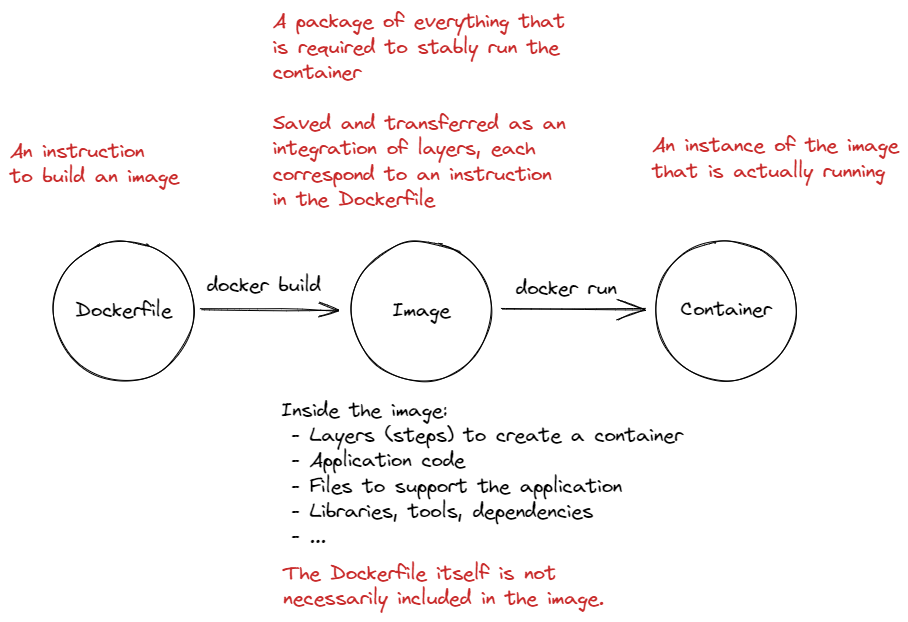
\includegraphics[width=350pt]{chapters/part-3/figures/dockerfiletoimage.png}
	\caption{A demonstration of how Dockerfile, image and container link to each other.} \label{ch:vac:fig:dockerfiletoimage}
\end{figure}

Since a docker image's primary role is to serve as a template for containers, many Dockerfile commands appear like a ``step-by-step'' recipe for container creation. Each instruction corresponds to an ``image layer''. An image is, in essence, an amalgamation of these layers. It is stored and distributed in this format. If images share layers (for instance, different versions of the same app), these shared layers are not saved or transferred redundantly, hence significantly reducing image sizes. More details can be found at \textit{https://docs.docker.com/storage/storagedriver/}.

\begin{shortbox}
\Boxhead{Docker Image Layers}

Docker containers employ a special file system known as the Union File System (UFS), which is well suited to the ``layer'' concept. UFS facilitates file sharing between the container and the host machine, along with combining read-only upper layers and writable lower layers, among other functions. 

A demonstration to illustrate this concept is given in Fig. \ref{ch:vac:fig:dockerlayerdemo}.

\end{shortbox}

\begin{figure}[!htb]
	\centering
	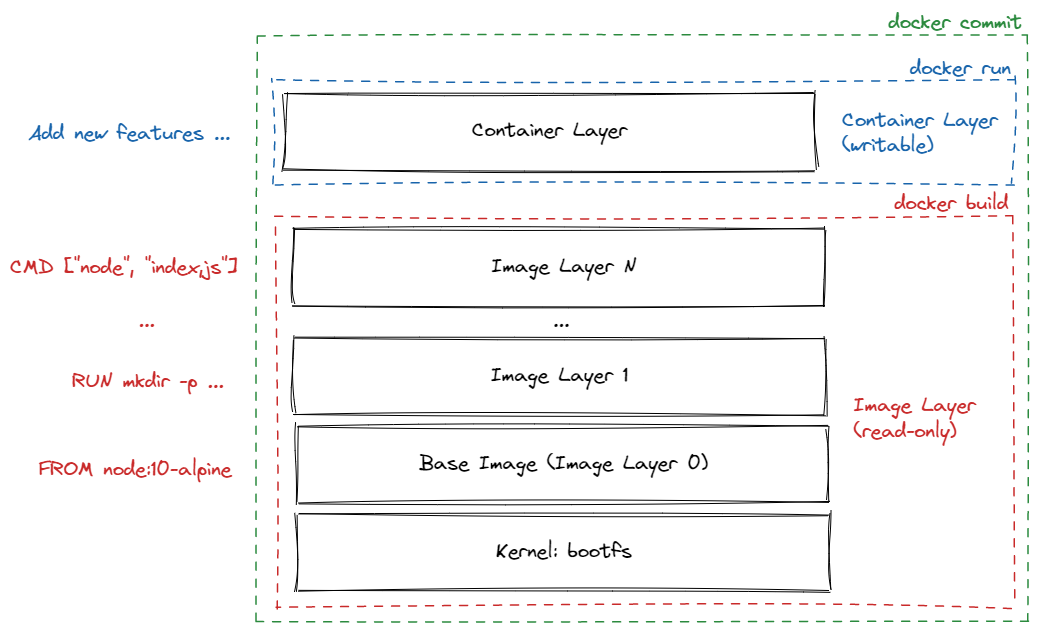
\includegraphics[width=350pt]{chapters/part-3/figures/dockerlayerdemo.png}
	\caption{A demonstration of docker image layer structure.} \label{ch:vac:fig:dockerlayerdemo}
\end{figure}

Just as a quick example, the Dockerfile to build the official \textit{hello-world} image from docker hub looks like the following.
\begin{lstlisting}
FROM scratch
COPY hello /
CMD ["/hello"]
\end{lstlisting}
In the example above, \verb|FROM scratch| signifies that this image is a base image without a parent. The \verb|COPY hello /| instruction copies the \textit{hello} binary script from the image to the root directory of the container. Lastly, \verb|CMD ["/hello"]| runs the \textit{hello} binary script.

In general, a typical Dockerfile includes the following instructions to build an image. These instructions allow the image to know how to create a container, automatically construct the file system directory structure, install necessary packages, and run the app:
\begin{enumerate}[(1)]
  \item Define parent image.
  \item Create filesystem directory.
  \item Set working directory.
  \item Copy files.
  \item Configure registry.
  \item Install packages.
  \item Copy more files after package installation.
  \item Switch to the correct user.
  \item Expose port.
  \item Run the application.
\end{enumerate}

The commonly used keywords to be used in a Dockerfile to realize the above instructions, such as \verb|FROM|, \verb|RUN|, are explained in Table \ref{ch:vac:tab:keywordsdockerfile}. 

It is worth highlighting the distinction between \verb|RUN| and \verb|CMD|. The \verb|RUN| command is executed during the building of the image, which creates a virtual representation of the environment to run the service. Therefore, \verb|RUN| is used to prepare the environment, for example, to install necessary libraries. On the other hand, command \verb|CMD| simply specifies the default command to run when the container starts. It is in built together with the image, but not considered as a read-only image layer. Indeed, the contents in \verb|CMD| can even be overwritten if the user wishes to do so when \verb|docker run| executes.

\begin{table}[!htb]
	\centering \caption{Critical keywords used in a Dockerfile.}\label{ch:vac:tab:keywordsdockerfile}
	\begin{tabularx}{\textwidth}{lX}
		\hline
		Syntax & Description \\ \hline
		\verb|FROM <image>[:<tag>]| & Define the base image. A Dockerfile must start with a \verb|FROM| instruction. In case of multiple \verb|FROM| instructions, the last one statement is the base image and the earlier ones intermediate images. An optional \verb|:<tag>| can be used to specify the version of the base image. \\ 
		\verb|RUN <command>| & Execute a shell command. \\ 
		\verb|WORKDIR <path>| & Set the working directory from the point onwards. \\ 
		\verb|ADD <src> <dest>| & Add (Copy) \verb|<src>|, either a directory/file or URL, to \verb|<dest>|. An optional \verb|[--chown=<user>:<group>]| can be used to specify the owner and group of the added files. \\ 
		\verb|COPY <src> <dest>| & Similar with \verb|ADD|. \verb|COPY| is easier but less powerful and cannot handle tar or URL. \\ 
		\verb|USER <user>| & Switch user from the point onwards. \\ 
		\verb|EXPOSE <port>| & Specifies the ports that the container shall listen to. An optional \verb|/<protocol>| can be used to specify the protocol for communication. \\
        \verb|VOLUME ["<path>"]| & Attaches an anonymous volume to the specified path inside the container. \\
		\verb|CMD ["<exe>", "<arg>",]| & The user-script command. This is the last instruction in the Dockerfile that usually starts the APP. Notice that a Dockerfile can only contain one \verb|CMD| instruction. The user script is included in the image but not as a the read-only layer. \\
		\hline
	\end{tabularx}
\end{table}

Besides Table \ref{ch:vac:tab:keywordsdockerfile}, there are other Dockerfile keywords that can significantly simplify the design and maintenance of the image. For example, \verb|ENV <key>=<value>| assign a value to an environmental variable which can later be referred as \verb|$<key>| in the Dockerfile. An example is given below.
\begin{lstlisting}
ENV PORT=80
EXPOSE $PORT # this is interpreted as EXPOSE 80
\end{lstlisting}
Notice that environmental variables are accessible by the application code. They can be overwritten during \verb|docker run|. This means that the user can potentially use environmental variable to dynamically change the behavior of the application in the container when using \verb|docker run|. There are several benefits of doing this, for example, to enhance security. For example, if there is a password that the user needs to key in during the start of the container, the developer may want to put it as environmental variable and let the user to fill in, instead of hardcode the password in Dockerfile.

Another useful features of Dockerfile is the Dockerfile argument. It leaves a ``space'' in the Dockerfile that the developer can later fill in when he builds the image. An example is given below.
\begin{lstlisting}
ARG DEFAULT_PORT[=80]
ENV $DEFAULT_PORT
EXPOSE $PORT
\end{lstlisting}
The default value \verb|[=80]| is optional. When building the image, use \verb|--build-arg <variable-name>=<value>| to override the argument value. Notice that unlike environmental variables, Dockerfile arguments are not accessible by the application code or by the \verb|CMD| instruction.

Additionally, \verb|LABEL <key>="<value>"| assigns a tag to the image, which can be displayed when \verb|docker inspect <container>| is used.

Dockerfile programming can be very flexible and complicated at the same time. The advanced materials goes beyond the scope of this notebook.

Examples of Dockerfiles are given below, one from \textit{docs.docker.com} and the other from Linux Academy. The docker image layer structure of the second example is given in Fig. \ref{ch:vac:fig:dockerlayerdemo} as a demonstration. Notice that in Fig. \ref{ch:vac:fig:dockerlayerdemo}, \verb|bootfs| refers to the ``boot file system'', including the bootloader and the Linux kernel. Upon creation of a container using \verb|docker run|, a container layer will be added to the image, as shown by the blue dashed box in Fig. \ref{ch:vac:fig:dockerlayerdemo}. In the container, all the changes made is saved into the container layer.

To generate a new image to include the changes made in the container, use \verb|docker commit|, which essentially commits the container layer as the latest image layer in the new image, as shown by the green dashed box in Fig. \ref{ch:vac:fig:dockerlayerdemo}.

\begin{lstlisting}
# First Example
FROM golang:1.16
WORKDIR /go/src/github.com/alexellis/href-counter/
RUN go get -d -v golang.org/x/net/html
COPY app.go ./
RUN CGO_ENABLED=0 GOOS=linux go build -a -installsuffix cgo -o app .

FROM alpine:latest
RUN apk --no-cache add ca-certificates
WORKDIR /root/
COPY --from=0 /go/src/github.com/alexellis/href-counter/app ./
CMD ["./app"]
\end{lstlisting}

\begin{lstlisting}
# Second Example
FROM node:10-alpine
RUN mkdir -p /home/node/app/node_modules && chown -R node:node /home/node/app
WORKDIR /home/node/app
COPY package*.json ./
RUN npm config set registry http://registry.npmjs.org/
RUN npm install
COPY --chown=node:node . .
USER node
EXPOSE 8080
CMD ["node", "index.js"]
\end{lstlisting}

With the Dockerfile ready, use \verb|docker build| to build an image. An example is given as follows.
\begin{lstlisting}
$ docker build <path/url> -t <image name>
\end{lstlisting}
or
\begin{lstlisting}
$ docker build <path/url> -t <user name>/<image name>:<tag>
\end{lstlisting}
where \verb|<path/url>| is the path or URL to the directory where the Dockerfile locates (does not need to contain ``\verb|/Dockerfile|'' in its end), and \verb|-t| gives a tag, in this case an image name, to the image to build. For the convenience of sharing, it is recommended that all images to be pushed to a public registry (such as Docker Hub) shall be tagged with user name and version. Notice that the tag can be changed later after the image is built.

It is worth mentioning that \verb|docker build| builds the images by layers in the Dockerfile, and it will not re-build the same layer to which point no changes are made. This feature suggests that we should put the common and static layers in the early part of Dockerfile, and customized and user-defined layers in the late part, thus making the building (and also sharing, as will be introduced later) of the images more efficient.

Use \verb|.dockerignore| to exclude any files that should not be built into the image. Such files may include caches, the Dockerfile itself, etc.

\subsection{Docker Image Management}

The most commonly used image operations can be categorized as follows.
\begin{itemize}
  \item Create an image.
  \item Create a container from an image.
  \item Upload and download an image from a remote server.
  \item Manage local images, such as listing down all images, deleting an image, etc.
\end{itemize}

The first two operations have been introduced in earlier sections. The third and last ones are introduced below. Use the following command to search for an image on the default remote repository server (Docker Hub).
\begin{lstlisting}
$ docker search <image name>
\end{lstlisting}
Use the following command to download or update an image from the default remote repository server as follows. Notice that different from \verb|docker run|, this command will not start a container from the image.
\begin{lstlisting}
$ docker pull <image name>
\end{lstlisting}
Notice that since images are stored by layers, if two images share common layers, it is unnecessary to pull the shared layers repeatedly when downloading the second image, if the first image already exists in the host machine. Command \verb|docker pull| is smart enough to automatically detect shared layers, and avoid duplicating download of layers.

Use the following commands to list down or remove images.
\begin{lstlisting}
$ docker image ls
$ docker image rm <image name>
$ docker rmi <image name> # same as docker image rm
$ docker image prune # remove all problematic images
$ docker image prune -a # remove all unused images
\end{lstlisting}
where \verb|prune| removes all problematic images, and \verb|prune -a| removes all unused images from local.

Use the following command to inspect an image, and list down its metadata details.
\begin{lstlisting}
$ docker image inspect <image name>
\end{lstlisting}

\subsection{Docker Image Sharing with Docker Hub}

There are two ways to share an image:
\begin{itemize}
	\item Share the Dockerfile and APP source code so that the receiver can build docker image from his end.
	\item Share the image directly.
\end{itemize}
It is often more convenient to share the built image instead of the Dockerfile and the source code. However, a docker image is stored and managed by layers and cannot be shared simply by file transfer. 

Docker Hub is a commonly used server for storing and sharing docker images. It is also the default remote repository server of docker engine. However, do notice that Docker Hub is not the only remote docker image server. Some alternatives are Amazon Elastic Container Registry, Red hat Quay, Azure Container Registry, Google Container Registry, etc.

After registering an account on docker bub, use the following command to login to the Docker Hub from your local machine.
\begin{lstlisting}
$ docker login --username=<user name>
Passowrd:
\end{lstlisting}

Assume that there is an image in the local machine, and an empty repository on Docker Hub. In order to push the local image to the Docker Hub, the first step is to add the remote repository and the ``\textit{RepoTags}'' in the local image as follows.
\begin{lstlisting}
$ docker tag <image name> <user name>/<repository name>:<version>
\end{lstlisting}
where \verb|<version>| is a tag usually used to distinguish the different branches or versions of the images on Docker Hub. For the first image upload, it can simply be \verb|latest|.

Use the following command to push the image to Docker Hub.
\begin{lstlisting}
$ docker push <user name>/<repository name>
\end{lstlisting}

Notice that when using \verb|docker run| on an image with out a specified version and the image is not stored locally, Docker will automatically search and pull the latest version of that image from the remote repository, usually Docker Hub by default. However, if the image already exists locally, Docker simply uses that image and will not automatically check the remote repository for the latest version. To update the local image, manually use \verb|docker pull| to pull the latest or specific version of the image from the remote repository.

\section{Multi-Container Deployment and Orchestration}

This section discusses the deployment and orchestration of multi-container applications. Different methods to enable container-to-host and container-to-container communications are introduced. Docker compose, a useful tool to automatically configure and start containers of a multi-container application, is also introduced.

\subsection{Communication}

In practice, a containerized application needs to communicate with applications running outside the container to request services such as API calls. Commonly seen use cases are as follows.
\begin{itemize}
	\item Containerized application requests services from the Internet.
	\item Containerized application requests services from the host machine, for example, from a database deployed on the host machine.
	\item Containerized application requests services from other containerized applications.
\end{itemize}

With proper port mapping using \verb|-p|, the communication with the Internet is automatically enabled. Therefore, the focus of this section is mainly on data exchange and API calls between the container and the host machine or other containers.

The containerized application may request services from the host machine. In this case, the application code needs to be modified to enable communications with the host machine. An example is given below.

Consider a simple scenario where the containerized application needs to send a request to the host machine to trigger an API call of MongoDB. Notice that the MongoDB is installed on the host machine and not in the container.

If the application were running on the host machine instead of in a container, it can communicate with the MongoDB server using a connecting string that looks like the following
\begin{lstlisting}
'mongodb://localhost:27017/<database name>'	
\end{lstlisting}
and it should be part of the application code. However, it would not work if the same code is used in the containerized application. The code needs to be modified as follows.
\begin{lstlisting}
'mongodb://host.docker.internal:27017/<database name>'	
\end{lstlisting}
where \verb|host.docker.internal| is a recognized domain by docker that refers to the host machine. Docker translates the domain to the IP address of the host machine.

Notice that \verb|host.docker.internal| can be used to refer to the host machine not only with MongoDB requests, but also with other requests such as a general HTTP request.

Two containers running on the same machine can always talk to each other via the host machine. However, this may become inefficient in some applications. Therefore, we need to investigate on direct container-to-container communication.

As a basic solution, cross container communication can be done following the example given below. Notice that this is not a common practice in production environment as it is not robust and efficient.

Consider a simple scenario where there are two containers, one running the application and the other hosting a MongoDB. 

The container with MongoDB deployment is started as follows.
\begin{lstlisting}
$ docker run -d --name mongodb mongo 	
\end{lstlisting}
where \verb|mongo| is the official docker image for MongoDB on Docker Hub.

The IP address of the MongoDB container can be found using
\begin{lstlisting}
$ docker container inspect mongodb	
\end{lstlisting}
where \verb|mongodb| is the name of the container specified in the earlier command. In the result of the inspection, look for \verb|IPAddress| under \verb|NetworkSettings|.

Then in the application code, replace \verb|localhost| in the connecting string
\begin{lstlisting}
'mongodb://localhost:27017/<database name>'	
\end{lstlisting}
with the IP address of the container.

Notice that each time a container is deployed, its network settings are done by docker and they differ from machine to machine. Therefore, this basic approach only works temporarily in development environment and should not be used in the production environment.

As a more established approach to realize cross container communication, docker allows the user to create container networks. All containers in a container network have reserved IP addresses assigned by docker and they can talk to each other.

To create a container network, use
\begin{lstlisting}
$ docker network create <network name>
\end{lstlisting}
Then to associate an container with that container network, use \verb|--network| as follows
\begin{lstlisting}
& docker run --network <network name>	<image name>
\end{lstlisting}
If two containers are put under the same container network, they can talk to each other. 

Consider the earlier example. We can create a container network using
\begin{lstlisting}
$ docker network create my-network
\end{lstlisting}
and launch MongoDB as a containerized application in the container network using
\begin{lstlisting}
$ docker run -d --network my-network --name mongodb mongo
\end{lstlisting}
In the application code, use
\begin{lstlisting}
'mongodb://mongodb:27017/<database name>'	
\end{lstlisting}
as the connecting string, and launch it in the same container network. Docker will automatically resolve \verb|mongodb| as the correct container with that container name when the application sends out the outbound request.

Notice that when using container network for cross container communication, there is no need to do port match using \verb|-p|. Indeed, \verb|-p| is used only when the container needs to talk to the outside world through the host machine. Cross container communication as well as container to host machine communication happens inside the host machine, thus not requiring port mapping.

\subsection{Docker Compose}

As introduced earlier, docker engine can be used to build and share images as well as start, monitor, and stop containers. It can be difficult for a user to manage containers manually when a lot of them are deployed. Container orchestrators such as Portainer and Kubernetes are helpful with managing containers. Many of these tools are able to automatically adjust the number of containers and balance their loads.

Many applications nowadays are multi-service multi-container applications. This trend has made container orchestration very useful in practice.

Consider building and launching a multi-container applications. Multiple \verb|docker build| and \verb|docker run| commands need to be executed in specific order, and each command coming with a long list of arguments. Doing this manually can be tedious and introduce a high chance of human error.

A docker compose file is essentially a configuration file in YAML, usually named \verb|docker-compose.yml| (in later versions of docker compose, it can also be named \verb|compose.yml|). It plays as the user script or configuration file that automate the processes. Docker compose can process that configuration file, then build and launch containers accordingly. From that sense, docker compose can be seen as a container orchestration tool. 

This section gives a brief introduction to the preparation of a docker compose file. Examples of docker compose files can be found elsewhere online, such as \texttt{github.com/docker/awesome-compose}. 

A typical docker compose file looks like the following.

\begin{lstlisting}
version: "<compose file format version>"
services:
  <container name 1>:
    image: "<image name>"
    container_name: "<container name>"
    volumes:
      - <volume name 1>:<container path> # named volume
      - <container path> # anonymous volume
      - <host path>:<container path> # bind mount
      - ...
    environment:
      - <variable name 1>=<value 1>
      - <variable name 2>=<value 2>
      - ...
    env_files:
      - <path to environmental variable file 1>
      - <path to environmental variable file 2>
      - ...
    networks:
      - <network name>
    ports:
      - "<host port>:<contianer post>"
  <container name 2>:
    build:
      context: <path to Dockerfile directory>
      dockerfile: <name of docker file>
    volumes:
      - <volume name 2>:<container path> # named volume
      - <container path> # anonymous volume
      - <host path>:<container path> # bind mount
      - ...
    environment:
      - <variable name 1>=<value 1>
      - <variable name 2>=<value 2>
      - ...
    env_files:
      - <path to environmental variable file 1>
      - <path to environmental variable file 2>
      - ...
    networks:
      - <network name>
    ports:
      - "<host port>:<contianer post>"
    depends_on:
      - <container name>
      - ...
volumes:
  <volume name 1>: # for named volumes only
  <volume name 2>:
  ...
\end{lstlisting}
Some highlights are as follows.
\begin{itemize}
	\item \verb|version| tells the the compose file format version. Docker compose will then parse the compose file accordingly. 
	
	Different compose file format version may support different fields. If the version field is omitted, the composed file is parsed according to the latest version.
	
	\item \verb|services| describes the container(s) to be deployed. Each container is corresponding with a subcomponent under services.
	
	For simple containers whose image is readily available without \verb|docker build|, the following fields are commonly used in the subcomponent.
	
	\begin{itemize}
		\item \verb|image| specifies the image.
		\item \verb|container_name| specifies the container name; if not specified, default names will be used which are still human-readable.
		\item \verb|volumes| defines volumes and bind mounts.
		\item \verb|environment| defines environmental variables. 
		\item \verb|env_file| includes a file inside which are environmental variables.
		\item \verb|networks| adds the service to a docker network. Notice that this is often not necessary as all the services will be automatically added to the same newly created default docker network by default, unless a network is specified.
		\item \verb|ports| maps host ports to container ports.
		\item \verb|depends_on| lists containers that need to be launched before the current container.
	\end{itemize}
	
	In the case where a new image needs to be built before launching the container, docker compose file requires the following fields to build the image.
	
	\begin{itemize}
		\item \verb|build| gives the paths to the docker file.
		
		\begin{itemize}
			\item \verb|context| gives the directory of the docker file. Everything to be built into the image must be in this directory or its subdirectories.
			\item \verb|dockerfile|: the name of the Dockerfile.
		\end{itemize}
		
		Notice that one can simply use \texttt{build: <context>} if Dockerfile is named \verb|Dockerfile|.
		
	\end{itemize}
	
	\item \verb|volumes| lists all the named volumes used by the services.
\end{itemize}

A docker compose file example is given below. This example is taken from \texttt{awesome-compose} on GitHub. 
\begin{lstlisting}
version: "3.8"
services:
  web:
    image: nginx
    volumes:
      - ./nginx/nginx.conf:/tmp/nginx.conf
    environment: 
      - FLASK_SERVER_ADDR=backend:9091  
    command: /bin/bash -c "envsubst < /tmp/nginx.conf > /etc/nginx/conf.d/default.conf && nginx -g 'daemon off;'" 
    ports:
      - 80:80
    depends_on:
      - backend
  backend:
    build:
      context: flask
      target: builder
    # flask requires SIGINT to stop gracefully
    # (default stop signal from Compose is SIGTERM)
    stop_signal: SIGINT
    environment:
      - FLASK_SERVER_PORT=9091
    volumes:
      - ./flask:/src
    depends_on:
      -  mongo  
  mongo:
    image: mongo
\end{lstlisting}

Finally, execute docker compose as follows.
\begin{lstlisting}
$ docker-compose up -d
\end{lstlisting}
if the docker compose file is named as the default name (usually \verb|docker-compose.yml|), or
\begin{lstlisting}
$ docker-compose -f <docker compose file name> up -d
\end{lstlisting}
if otherwise. Docker images shall be built and containers be launched accordingly. And to shutdown all the services, simply use
\begin{lstlisting}
$ docker-compose down
\end{lstlisting}

Docker compose would not re-build the images by default if it thinks that the images it will use have been built before. To enforce rebuild, consider using \verb|--build| flag. Alternatively, use 
\begin{lstlisting}
$ docker-compose build
\end{lstlisting}
to build the images in the docker compose file without launching any container.

\section{Container Cloud Deployment}

So far we have been discussing container development and local testing. One of the most important selling points of containerization is that it is easy to ship applications. This is because the environment that supports an application is packaged together with the application in the image, which ensures that the application can run consistently whatever the host server is. 

Nevertheless, when the application is pushed to production environment, some adjustments need to be made. To name a few, below is a list of probable adjustments when shipping from development to production.

\begin{itemize}
	\item Bind mounts should not be used. Use \verb|COPY| to encapsulate all the resources needed, and use volume if data persistence is required.
	\item Some container setups may need to be changed.
	\item For multi-container applications, the containers may need to be deployed on multiple hosts.
\end{itemize}

This section discusses the deployment of containers on the cloud in production environment. Notice that for large scale applications deployment in the production environment, container orchestration tool such as Kubernetes is almost certainly necessary. Kubernetes and its cloud deployment are discussed in the later chapter and they are not considered in this section. 

\subsection{Docker Hosting Providers}

Assume that the application can run correctly on the host machine. To deploy it on the Internet and allow public access, the first step is to find a docker-supporting hosting provider. There are many such providers, the most popular of which include Amazon Web Services (AWS), Microsoft Azure and Google Cloud. They are not just docker hosting providers but more general cloud services providers.

Details about the cloud services providers and cloud computing are beyond the scope of this notebook. Only the services relevant to container deployment are introduced here. AWS is considered.

\subsection{VM-Based Approach}

The most intuitive way to deploy containers on AWS is to use EC2, the VM as part of AWS's IaaS solution. To do that, the following steps are required.

\begin{enumerate}
	\item Start EC2, and enable SSH access to the EC2 from the local machine.
	\item Install docker on the EC2 instance.
	\item Upload the images which have been built in the local machine to the EC2 instance.
	\item Start the containers on EC2.
	\item Enable public access to the EC2 by publishing its IP address.
\end{enumerate}

Notice that EC2-based deployment is not the best practice as AWS and many other cloud service providers have managed container management services such as Elastic Container Service (ECS) and Elastic Kubernetes Service (EKS). However, for illustration purpose, we will start from EC2-based deployment.

The key steps to launch and connect to a EC2 instance from a Linux local machine are given below.
\begin{enumerate}
  \item Create and configure the EC2 instance from AWS dashboard.
  \item In the last step of EC2 instance configuration, create or select a key pair. The key pair is used later to SSH to the instance. Download the private key pair. The name of the private key pair is by default \verb|<key pair name>.pem|. 
  \item Change the ACL of the private key pair to \verb|400| to disable public view using \texttt{chmod 400 <key pair name>.pem}.
  \item Launch the EC2 instance from AWS dashboard. Wait until the instance state becomes ``running''. Locate the public DNS of the instance from the dashboard which usually looks like \texttt{<serial number>.<region>.compute.amazonaws.com}.
  \item SSH to the EC2 instance using \texttt{ssh -i "<key pair name>.pem" <username>@<public dns>}.
\end{enumerate}
To install and start docker on the EC2 instance, use
\begin{lstlisting}
$ sudo yum update -y
$ sudo yum install docker
$ sudo systemctl start docker
\end{lstlisting}
To upload an image from the local machine to the EC2 instance, use Docker Hub as a bridge. The user can then launch containers on the EC2 instance the same way he would do on a local machine. Lastly, to enable public access to the EC2 from HTTP, configure the security group inbound rules attached to the EC2 instance. By default, the only allowed inbound rule is SSH using TCP protocal via port range 22 from all IP addresses. Depending on the applications running on the EC2 instance, the user may want to add more inbound rules, for example, enabling HTTP/HTTPS access via port 80.

For multi-container applications, the user can upload all necessary images to Docker Hub, and on the EC2 instance simply execute a docker compose file. Notice that the docker compose file should use the images on Docker Hub instead of building any on the fly. In production environment, all the images should be pre-built.

The EC2-based approach has some disadvantages compared with ECS and EKS that will be introduced in later sections. There are at least the following disadvantages.
\begin{itemize}
  \item Lack of robustness. EC2 belongs to the Infrastructure as a Service (IaaS) family where AWS only supports the infrastructure (in this case, the VM) and not anything running on it (in this case, docker and the containerized application). The user needs to deal with all the ``accidents'' that may break the system such as someone launching a cybor attack on the VM. This makes the solution less robust.
  \item Difficult to scale. The total computational power of the application depends on the setup of VM which is pre-determined and cannot be easily scaled up or down on the fly.
  \item Difficult to manage. The user needs to SSH to the VM to audit and upgrade the applications, which can become annoying.
\end{itemize}
This makes EC2-based container approach almost always suboptimal compared with ECS and EKS, especially if the user is not an experienced administrator.

\subsection{Managed-Service-Based Approach}

ECS and EKS are the recommended manages service of AWS for containerized applications. EKS will be introduced in the later chapter with Kubernetes. This section discusses ECS. Notice that when using a managed service like ECS, it is no longer the user's concern what container runtime or engine the managed service is using in the backend. The user does not need (and should not) interact with docker directly. Instead, he should use the interface ECS provides.

As a prerequisite, make sure that the images to be used are already in Docker Hub. 

\vspace{0.1in}
\noindent \textbf{Single-Container Applications}
\vspace{0.1in}

Key steps to deploy containerized applications using ECS are summarized below. The user needs to configure ``container'', ``task'', ``service'' and ``cluster'' to be used for the application.

Container defines how a container should be launched. In container definition, the following items need to be configured.
\begin{itemize}
  \item Container name.
  \item Image path. If the image has been uploaded to Docker Hub, use \texttt{<username>/<image>:<tag>}.
  \item Memory limit.
  \item Port mapping.
  \item If health check is necessary, health check related configurations such as timeout, number of retires, etc.
  \item If the default \verb|CMD| needs to be overwritten when starting the container, the command to overwrite \verb|CMD|.
  \item If the default \verb|WORKDIR| needs to be overwritten, the revised working directory path.
  \item The value of environmental variables, if any.
  \item Network configuration.
  \item Volume configuration.
  \item Log configuration.
  \item \ldots
\end{itemize}
One can think of most of the above as the customization of \verb|docker run| command which has already been introduced in earlier sections.

Task defines the server requirements that host the containers. The user needs to define task definition name, network model, compatibilities request, etc. For example, in compatibilities if ``FARGATE'' is selected, AWS runs the containers in a serverless manner, whereas if ``EC2'' is selected, AWS creates dedicated VMs to run the containers.

Service plays as the ``orchestrator'' of tasks. It defines the number of tasks to be used and how load is balanced among the tasks.

Finally, cluster defines the virtual private cloud (VPC) and subnets where the application should be running, as part of the network configuration in AWS architecture. Cluster definition is important if multiple applications need to be run under the same virtual network, or if the application needs to access certain resources inside certain VPC.

Once all the configurations above are done properly, ECS will start the application. From the dashboard, one can get the public IP address of the task where the containers are hosted, and access the containers using that IP.

To update the image, go to ``Task Definitions'', click ``Actions'', and choose ``Update Service'', ``Force New Deployment''. AWS will then retrieve the new image and restart the task. Of course, one can always start a new task, in which case EC2 will also retrieve the new image. 

\vspace{0.1in}
\noindent \textbf{Multi-Container Applications}
\vspace{0.1in}


On the local machine or the VM, multi-container applications can be launched easily using docker compose. ECS also supports the launch of multi-container applications. 

However, ECS does not use docker compose file to start multi-container applications. One of the reasons for that is that docker compose assumes single physical machine deployment, hence supporting all the notions that the user can use to setup networks, volumes, etc. This is not the case of ECS which does not necessarily deploy everything on one host. This makes the docker compose file less relevant. Nevertheless, the docker compose file, if already exists, can be used as a blue print and the user can refer to the file when deploying containers using ECS.

In ECS, if multiple containers are assigned to the same task, then they are guaranteed to run on the same machine and under the same network. In that case, the application can use \verb|localhost| to communicate with other containers, where \verb|localhost| can be taken as a docker container created for all the containers running on the task. (Recall that to enable container-to-container communication on a local machine, \verb|localhost| in the application code needs to be changed to either the IP address of the container, or the name of the container if they are in the same docker network.)























